\subsection{Correlations and Clustering between the Implied and the Realised Volatility}
A simple scatter plot of the implied volatility and the realised volatility reveals interesting very insights. Note that sample is limited to 50-Delta options.

\begin{figure}[H]
    \centering
    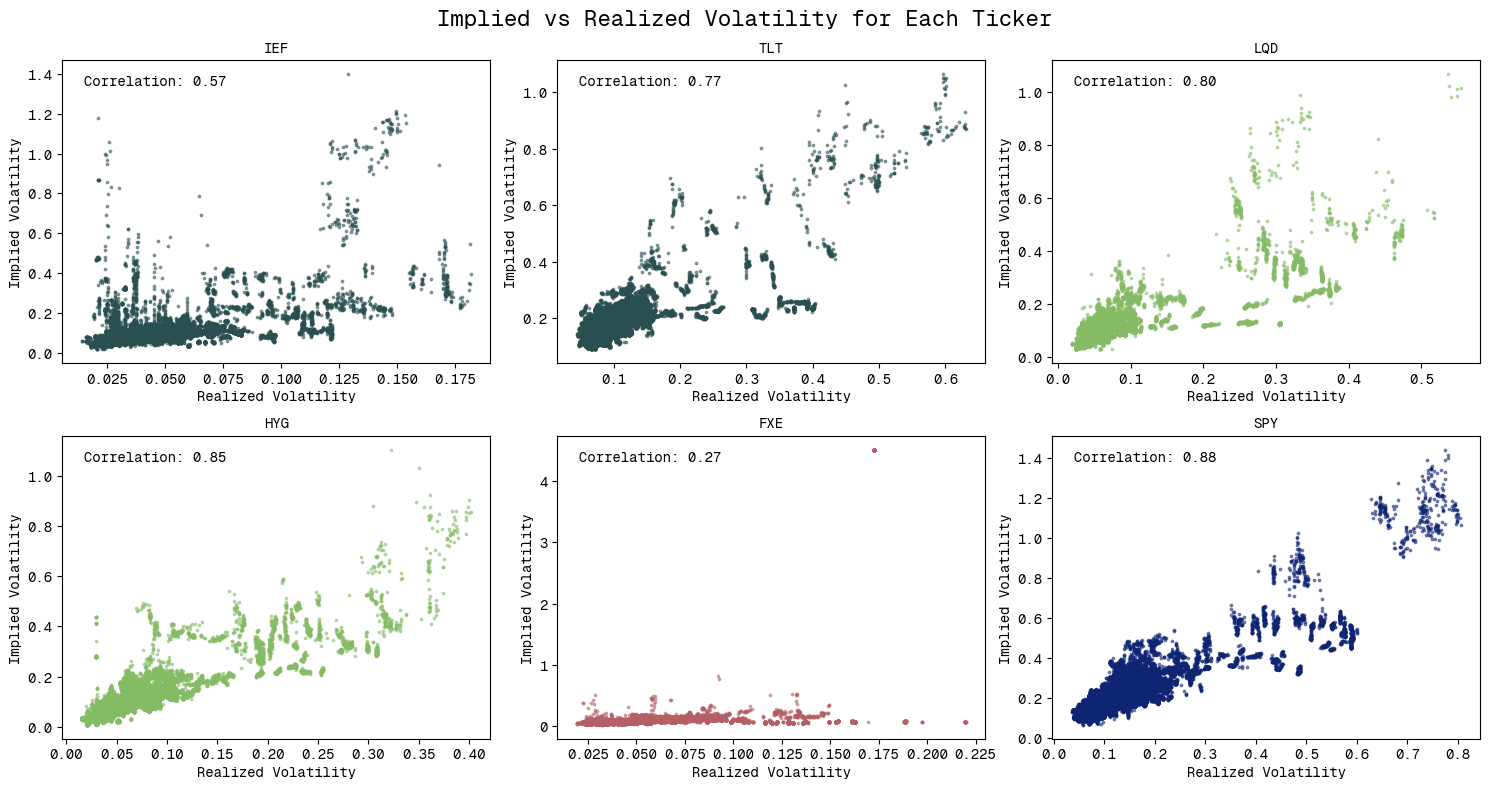
\includegraphics[width=1\textwidth]{images/iv_and_rv_batch1.png}
    \caption{Implied and the Realised Volatility}
    \label{fig:iv_and_rv1}
\end{figure}

We find a very high correlation between implied volatility (IV) and realized volatility (RV) for iShares 20+ Year Treasury Bond ETF (TLT), iShares iBoxx \$ Investment Grade Corporate Bond ETF (LQD), SPDR S\&P 500 ETF Trust (SPY), and iShares iBoxx \$ High Yield Corporate Bond ETF (HYG). However, CurrencyShares Euro Trust (FXE) stands out. Contrary to other tickers, it is the only one that exhibits extremely low correlation. Another interesting phenomenon is the clustering of points at the north-east corner of SPDR S\&P 500 ETF Trust (SPY) ticker. It appears as if the implied volatility tends to overshoot once a certain threshold of realized volatility has been crossed for this ticker. What explains this phenomenon could be an interesting research question and a hot-bed for a machine learning predictive model. A similar clustering is also observed for the small-cap index - iShares Russell 2000 ETF (IWM) and shiny metals (GLD and SLV).

\begin{figure}[H]
    \centering
    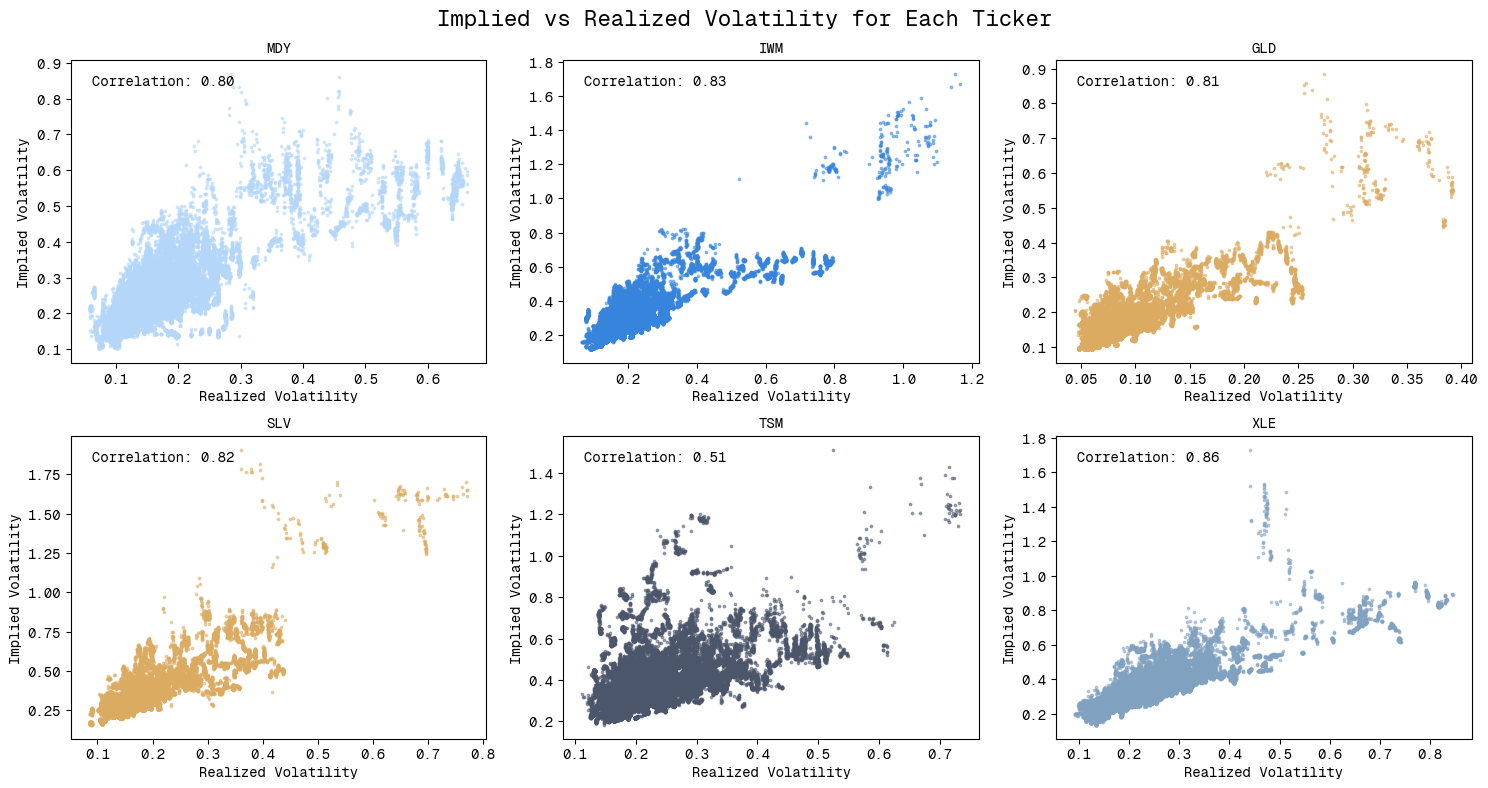
\includegraphics[width=1\textwidth]{images/iv_and_rv_batch2.png}
    \caption{Implied and the Realised Volatility}
    \label{fig:iv_and_rv2}
\end{figure}

The insights turn even more interesting when we look at OTM call options that is the contracts with deltas between 0.2 and 0.3. The high correlation vanishes for almost every ticker. However, what is common is a cone like shape for almost every ticker. The interpretation is that when the realised volatility is low the implied volatilities are clustered at the lower end in a narrow area. As the uncertainty increases, the range of implied volatilities that are observed becomes wider. 

\begin{figure}[H]
    \centering
    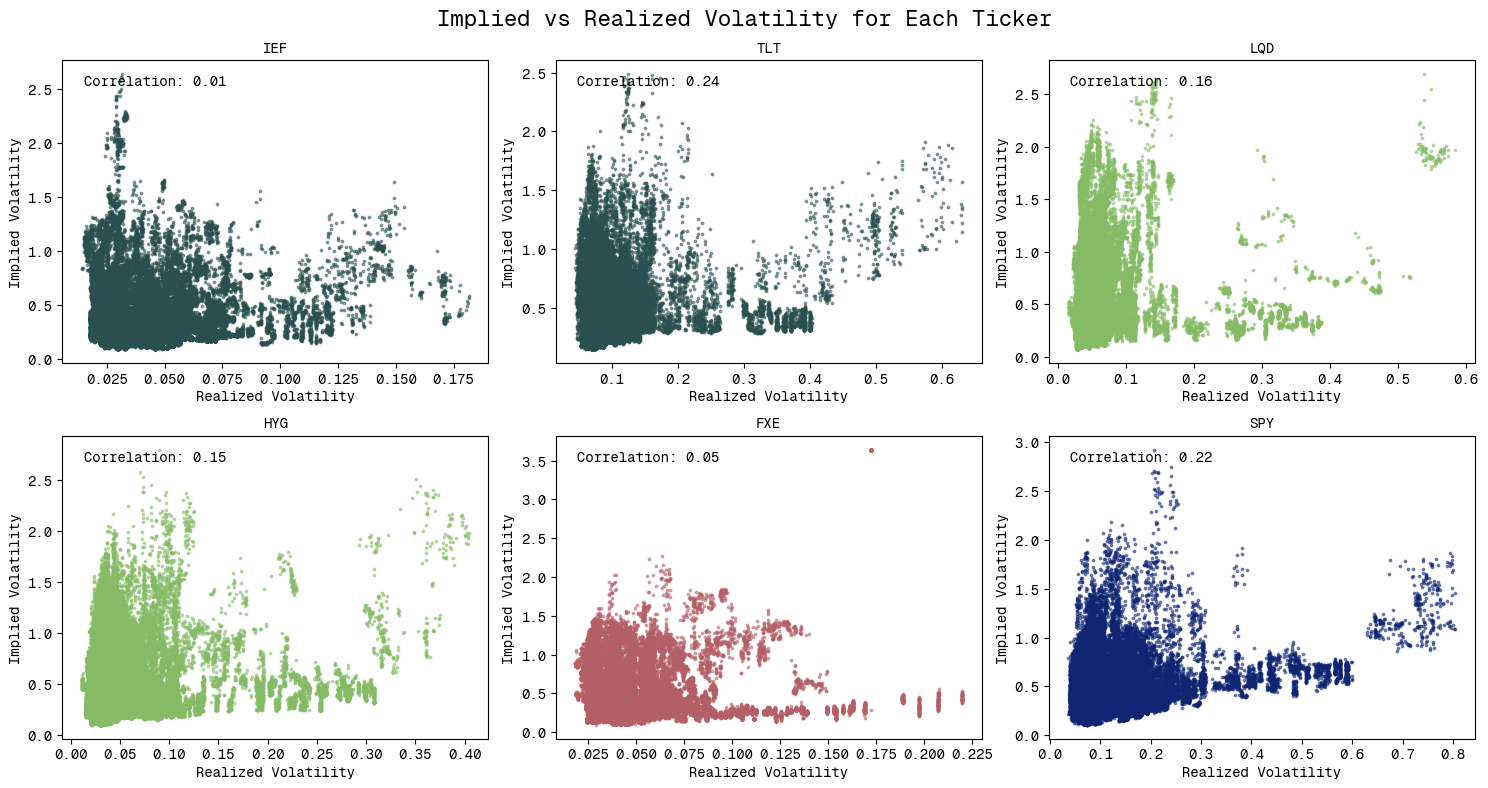
\includegraphics[width=1\textwidth]{images/iv_and_rv_otm_batch1.png}
    \caption{Implied and the Realised Volatility}
    \label{fig:iv_and_rv__otm_1}
\end{figure}

\begin{figure}[H]
    \centering
    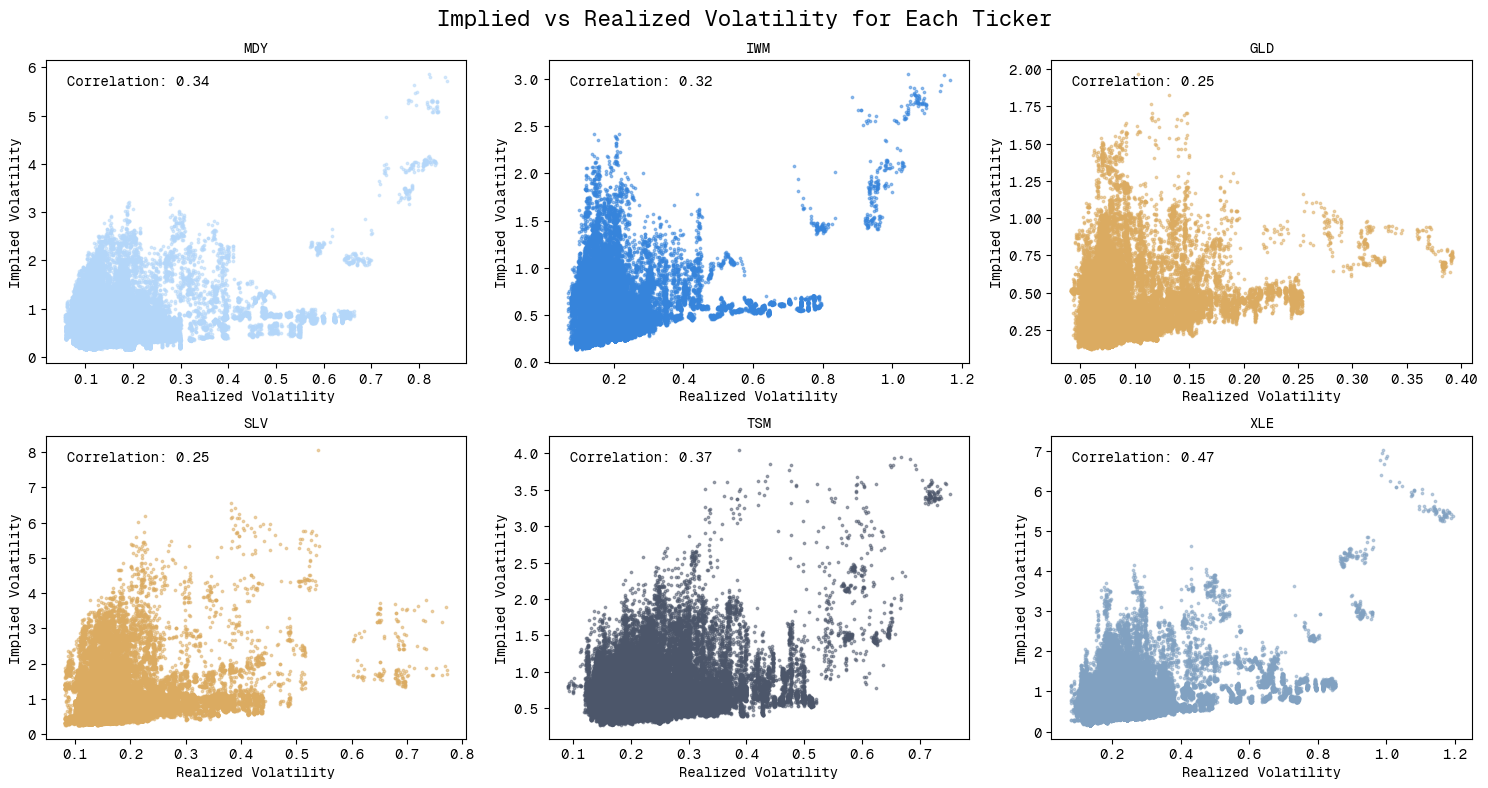
\includegraphics[width=1\textwidth]{images/iv_and_rv_otm_batch2.png}
    \caption{Implied and the Realised Volatility}
    \label{fig:iv_and_rv__otm_2}
\end{figure}

Now having looked at the joint distributions of IV and RC, we will move on to the volatility risk premium.